% Options for packages loaded elsewhere
\PassOptionsToPackage{unicode}{hyperref}
\PassOptionsToPackage{hyphens}{url}
\PassOptionsToPackage{dvipsnames,svgnames,x11names}{xcolor}
%
\documentclass[
<<<<<<< HEAD
  8.5pt,
  letterpaper,
]{article}

\usepackage{amsmath,amssymb}
\usepackage{lmodern}
=======
  9pt,
  letterpaper,
  DIV=11,
  numbers=noendperiod]{scrartcl}

\usepackage{amsmath,amssymb}
>>>>>>> 0324c0dd673a4473a6c11ce2d1afb0ef56d69683
\usepackage{setspace}
\usepackage{iftex}
\ifPDFTeX
  \usepackage[T1]{fontenc}
  \usepackage[utf8]{inputenc}
  \usepackage{textcomp} % provide euro and other symbols
\else % if luatex or xetex
  \usepackage{unicode-math}
  \defaultfontfeatures{Scale=MatchLowercase}
  \defaultfontfeatures[\rmfamily]{Ligatures=TeX,Scale=1}
\fi
<<<<<<< HEAD
=======
\usepackage{lmodern}
\ifPDFTeX\else  
    % xetex/luatex font selection
\fi
>>>>>>> 0324c0dd673a4473a6c11ce2d1afb0ef56d69683
% Use upquote if available, for straight quotes in verbatim environments
\IfFileExists{upquote.sty}{\usepackage{upquote}}{}
\IfFileExists{microtype.sty}{% use microtype if available
  \usepackage[]{microtype}
  \UseMicrotypeSet[protrusion]{basicmath} % disable protrusion for tt fonts
}{}
\usepackage{xcolor}
<<<<<<< HEAD
\usepackage[lmargin=0.25in,rmargin=0.25in,tmargin=0in,bmargin=0.5in]{geometry}
=======
\usepackage[lmargin=0.25in,rmargin=0.25in,tmargin=0in,bmargin=0.25in]{geometry}
>>>>>>> 0324c0dd673a4473a6c11ce2d1afb0ef56d69683
\setlength{\emergencystretch}{3em} % prevent overfull lines
\setcounter{secnumdepth}{-\maxdimen} % remove section numbering
% Make \paragraph and \subparagraph free-standing
\ifx\paragraph\undefined\else
  \let\oldparagraph\paragraph
  \renewcommand{\paragraph}[1]{\oldparagraph{#1}\mbox{}}
\fi
\ifx\subparagraph\undefined\else
  \let\oldsubparagraph\subparagraph
  \renewcommand{\subparagraph}[1]{\oldsubparagraph{#1}\mbox{}}
\fi


\providecommand{\tightlist}{%
  \setlength{\itemsep}{0pt}\setlength{\parskip}{0pt}}\usepackage{longtable,booktabs,array}
\usepackage{calc} % for calculating minipage widths
% Correct order of tables after \paragraph or \subparagraph
\usepackage{etoolbox}
\makeatletter
\patchcmd\longtable{\par}{\if@noskipsec\mbox{}\fi\par}{}{}
\makeatother
% Allow footnotes in longtable head/foot
\IfFileExists{footnotehyper.sty}{\usepackage{footnotehyper}}{\usepackage{footnote}}
\makesavenoteenv{longtable}
\usepackage{graphicx}
\makeatletter
\def\maxwidth{\ifdim\Gin@nat@width>\linewidth\linewidth\else\Gin@nat@width\fi}
\def\maxheight{\ifdim\Gin@nat@height>\textheight\textheight\else\Gin@nat@height\fi}
\makeatother
% Scale images if necessary, so that they will not overflow the page
% margins by default, and it is still possible to overwrite the defaults
% using explicit options in \includegraphics[width, height, ...]{}
\setkeys{Gin}{width=\maxwidth,height=\maxheight,keepaspectratio}
% Set default figure placement to htbp
\makeatletter
\def\fps@figure{htbp}
\makeatother

<<<<<<< HEAD
\usepackage[pages=some]{background}
% \usepackage{blindtext}
% \usepackage[fontsize=9.5pt]{fontsize}
=======

\usepackage[fontsize=9.5pt]{fontsize}
>>>>>>> 0324c0dd673a4473a6c11ce2d1afb0ef56d69683

\RedeclareSectionCommand[font=\centering\large]{section}
\RedeclareSectionCommand[
  runin=false,
  afterindent=false,
  font = \normalfont\textbf,
  beforeskip=1pt,
  afterskip=1pt]{subsection}

\setlength{\itemsep}{1pt}
\setlength{\parskip}{0pt}
\setlength{\parsep}{0pt}
\setlength{\labelsep}{0pt}
\setlength{\topsep}{0pt}
\setlength{\parsep}{0pt}
\setlength{\partopsep}{0pt}
\usepackage{fontspec}
\usepackage{multirow}
\usepackage{multicol}
\usepackage{colortbl}
\usepackage{hhline}
\newlength\Oldarrayrulewidth
\newlength\Oldtabcolsep
\usepackage{longtable}
\usepackage{array}
\usepackage{hyperref}
\usepackage{float}
\usepackage{wrapfig}
<<<<<<< HEAD
=======
\KOMAoption{captions}{tableheading}
>>>>>>> 0324c0dd673a4473a6c11ce2d1afb0ef56d69683
\makeatletter
\makeatother
\makeatletter
\makeatother
\makeatletter
\@ifpackageloaded{caption}{}{\usepackage{caption}}
\AtBeginDocument{%
\ifdefined\contentsname
  \renewcommand*\contentsname{Table of contents}
\else
  \newcommand\contentsname{Table of contents}
\fi
\ifdefined\listfigurename
  \renewcommand*\listfigurename{List of Figures}
\else
  \newcommand\listfigurename{List of Figures}
\fi
\ifdefined\listtablename
  \renewcommand*\listtablename{List of Tables}
\else
  \newcommand\listtablename{List of Tables}
\fi
\ifdefined\figurename
  \renewcommand*\figurename{Figure}
\else
  \newcommand\figurename{Figure}
\fi
\ifdefined\tablename
  \renewcommand*\tablename{Table}
\else
  \newcommand\tablename{Table}
\fi
}
\@ifpackageloaded{float}{}{\usepackage{float}}
\floatstyle{ruled}
\@ifundefined{c@chapter}{\newfloat{codelisting}{h}{lop}}{\newfloat{codelisting}{h}{lop}[chapter]}
\floatname{codelisting}{Listing}
\newcommand*\listoflistings{\listof{codelisting}{List of Listings}}
\makeatother
\makeatletter
\@ifpackageloaded{caption}{}{\usepackage{caption}}
\@ifpackageloaded{subcaption}{}{\usepackage{subcaption}}
\makeatother
\makeatletter
<<<<<<< HEAD
\@ifpackageloaded{tcolorbox}{}{\usepackage[many]{tcolorbox}}
=======
\@ifpackageloaded{tcolorbox}{}{\usepackage[skins,breakable]{tcolorbox}}
>>>>>>> 0324c0dd673a4473a6c11ce2d1afb0ef56d69683
\makeatother
\makeatletter
\@ifundefined{shadecolor}{\definecolor{shadecolor}{rgb}{.97, .97, .97}}
\makeatother
\makeatletter
\makeatother
<<<<<<< HEAD
=======
\makeatletter
\makeatother
>>>>>>> 0324c0dd673a4473a6c11ce2d1afb0ef56d69683
\ifLuaTeX
  \usepackage{selnolig}  % disable illegal ligatures
\fi
\IfFileExists{bookmark.sty}{\usepackage{bookmark}}{\usepackage{hyperref}}
\IfFileExists{xurl.sty}{\usepackage{xurl}}{} % add URL line breaks if available
\urlstyle{same} % disable monospaced font for URLs
\hypersetup{
  pdftitle={Longfin Inshore Squid () Ecosystem \& Socioeconomic Profile Report Card},
  colorlinks=true,
  linkcolor={blue},
  filecolor={Maroon},
  citecolor={Blue},
  urlcolor={Blue},
  pdfcreator={LaTeX via pandoc}}

\title{Longfin Inshore Squid (\protect\textit{Doryteuthis pealeii})
<<<<<<< HEAD
\protect\newline Ecosystem \& Socioeconomic Profile Report Card}
=======
\linebreak Ecosystem \& Socioeconomic Profile Report Card}
>>>>>>> 0324c0dd673a4473a6c11ce2d1afb0ef56d69683
\author{}
\date{}

\begin{document}
\maketitle
<<<<<<< HEAD
\ifdefined\Shaded\renewenvironment{Shaded}{\begin{tcolorbox}[borderline west={3pt}{0pt}{shadecolor}, interior hidden, enhanced, breakable, sharp corners, boxrule=0pt, frame hidden]}{\end{tcolorbox}}\fi
=======
\ifdefined\Shaded\renewenvironment{Shaded}{\begin{tcolorbox}[borderline west={3pt}{0pt}{shadecolor}, interior hidden, enhanced, boxrule=0pt, sharp corners, breakable, frame hidden]}{\end{tcolorbox}}\fi
>>>>>>> 0324c0dd673a4473a6c11ce2d1afb0ef56d69683

\setstretch{1}
\backgroundsetup{
  scale=1,
  angle=0,
  opacity=0,
  contents={
\includegraphics[width=\paperwidth,height=\paperheight]{bg_pg1.jpg}}
 }
\BgThispage

<<<<<<< HEAD
\vspace{-2.0cm}

\section{Spring 2026}

\vspace{0.75cm}

=======
\vspace{-0.5cm}
\section{Spring 2026}

>>>>>>> 0324c0dd673a4473a6c11ce2d1afb0ef56d69683
\begin{figure}

\begin{minipage}[t]{0.57\linewidth}

{\centering 

<<<<<<< HEAD
=======
\vspace{0.5cm}
>>>>>>> 0324c0dd673a4473a6c11ce2d1afb0ef56d69683
\raggedright
\section{Key Findings from the Life History Working Group}

\subsection{Lifespan and aging}

Growth is estimated to be 1 statolith ring/day, per multiple literature
sources. Participants at the longfin squid summit estimated a maximum
age of 15 months. Literature review supports a lifespan of less than 1
year. Recent (2024) statolith aging indicates maximum ages of 7 months
<<<<<<< HEAD
for females and 8.6 months for males (right) from squid caught in the
fishery.

\vspace{0.25cm}

\subsection{Maturity (from SQUIBS)}

In 2024, most stage 4 squid caught in summer with very little mature
squid caught the rest of the year. Highest numbers of immature (stage 1)
squid were caught in the second half of 2024. In 2025 (Jan-Apr), squid
caught represent largely intermediate maturity stages (2+3) with few
stage 1 and stage 4. Of 912 squid assessed, the dominant maturity stage
in females increases from Fall (1) -\textgreater{} Winter (2)
-\textgreater{} Spring (3). The highest percentage of mature male squid
were caught in spring and summer. No stage 4 females and very few stage
1 males were caught.
=======
for females and 8.6 months for males (right).
>>>>>>> 0324c0dd673a4473a6c11ce2d1afb0ef56d69683

\vspace{0.25cm}

\subsection{Migration and movement dynamics}

<<<<<<< HEAD
Literature review and recent work by Dave Richardson suggests the
possibility of a winter cohort that hatches south of Cape Hatteras and
subsequently migrates onto the Northeast U.S. continental shelf. Fishery
observations describe a spatial gradient of 1-6 cm mantle length (ML)
squid from waters south of Hatteras through southern New England, with
the smallest squid detected further south. The Gulf Stream and warm core
rings may facilitate the recruitment transport of juvenile squid
(Richardson WP).
=======
Literature suggests the possibility of a winter cohort that hatches
south of Cape Hatteras and subsequently migrates onto the Northeast U.S.
continental shelf. Fishery observations describe a spatial gradient of
1-6 cm mantle length (ML) squid from waters south of Hatteras through
southern New England, with the smallest squid detected further south.
The Gulf Stream and warm core rings may facilitate the recruitment
transport of juvenile squid (Richardson WP).
>>>>>>> 0324c0dd673a4473a6c11ce2d1afb0ef56d69683

\vspace{0.25cm}

\subsection{Reproductive dynamics}

Consideration of the hypothesis of a winter cohort spawning south of
Hatteras indicates the presence of multiple cohorts of longfin squid,
with some outside of the traditional Northeast shelf stock area, and
provides evidence of year-round spawning in the stock.

\vspace{0.25cm}

\subsection{Natural mortality}

Although natural mortality is expected to be age-dependent, lack of
accurate age data makes further study difficult. Multiple natural
mortality approximations could be developed to match lifespan
hypotheses. Intraspecific predation impacts natural mortality, but there
is no available data to quantify the amount of mortality this causes.

<<<<<<< HEAD
\vspace{1.0cm}

\includegraphics{/home/atyrell/SOE_ESP_Data/longfinESP/images/0521_conceptual model.png}
=======
\vspace{0.5cm}

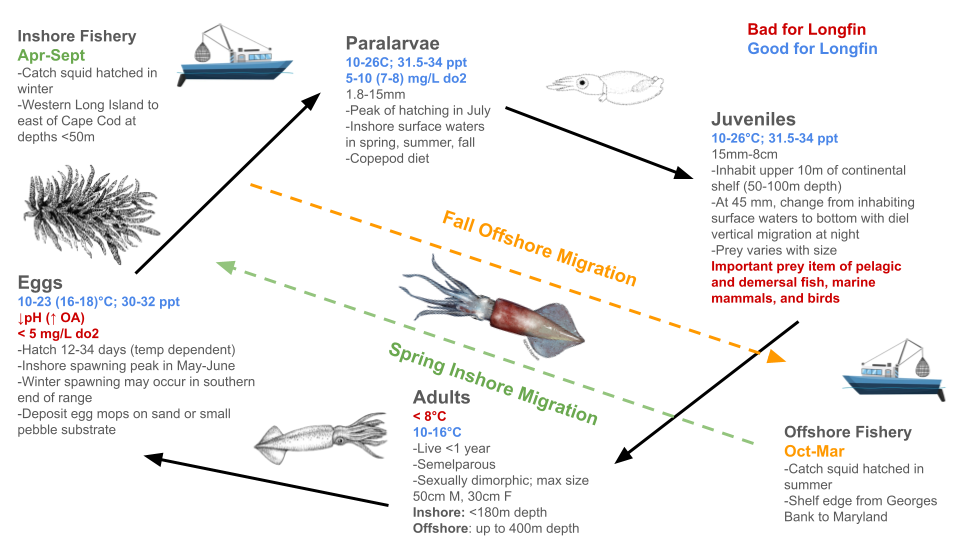
\includegraphics{C:/Users/stephanie.owen/Documents/longfinESP/images/conceptual_model.png}
>>>>>>> 0324c0dd673a4473a6c11ce2d1afb0ef56d69683

}

\end{minipage}%
%
\begin{minipage}[t]{0.03\linewidth}

{\centering 

\hfill

}

\end{minipage}%
%
\begin{minipage}[t]{0.40\linewidth}

{\centering 

<<<<<<< HEAD
\section{Longfin Squid Age Frequency from SQUIBS dataset}

\includegraphics{/home/atyrell/SOE_ESP_Data/longfinESP/images/squibs_data.png}

\vspace{1.0cm}
=======
\vspace{0.5cm}
\section{Longfin Squid Age Frequency from SQUIBS dataset}

\includegraphics{C:/Users/stephanie.owen/Documents/longfinESP/images/squibs_data.png}

\vspace{0.25cm}
>>>>>>> 0324c0dd673a4473a6c11ce2d1afb0ef56d69683

\section{Key Points from the Mid-Atlantic Risk Assessment}

\raggedright

In the
\href{https://static1.squarespace.com/static/511cdc7fe4b00307a2628ac6/t/67d45b1680e8654ecaf1b98e/1741970199497/b_Draft+MAB_RiskAssess_2025.pdf}{2025
Mid-Atlantic EAFM Risk Assessment Update}, longfin squid scored
moderate-high risk in the following elements:

\begin{itemize}
\tightlist
\item
  Moderate-high risk to the stock due to:

  \begin{itemize}
  \tightlist
  \item
    High potential for and observed distribution shifts\\
  \end{itemize}
\item
  Moderate-high risk to the commercial fishery due to:

  \begin{itemize}
  \tightlist
  \item
    Risk of not achieving optimum yield due to interactions with
    non-Council managed species
  \item
    Occasional recent changes in regulations; low-moderate regulatory
    complexity
  \item
    Regular, managed discards and incidental catch; moderate discard
    mortality
  \end{itemize}
<<<<<<< HEAD
\item
  Moderate-high risk to commercial fishery value

  \begin{itemize}
  \tightlist
  \item
    As it pertains to maximizing commercial fishery value based on net
    revenue and revenue, cost, and profitability indice findings
  \end{itemize}
\item
  Moderate-high risk to Commercial Fishery Resilience
  \textless80\textgreater\textless93\textgreater{} Fleet Diversity

  \begin{itemize}
  \tightlist
  \item
    Driven by 21 year down-ward trend of the Mid-Atlantic Fleet Count
    indicator
  \end{itemize}
\end{itemize}

\vspace{0.5cm}

\includegraphics{/home/atyrell/SOE_ESP_Data/longfinESP/images/risk_chart.png}
=======
\end{itemize}

\vspace{0.25cm}

\includegraphics{C:/Users/stephanie.owen/Documents/longfinESP/images/risk_chart.png}
>>>>>>> 0324c0dd673a4473a6c11ce2d1afb0ef56d69683

}

\end{minipage}%

\end{figure}

\newpage

\backgroundsetup{
  contents={
\includegraphics[width=\paperwidth,height=\paperheight]{bg_pg2.jpg}}
  }
\BgThispage

\newgeometry{top=0.25in, left=0.25in, right=0.25in, bottom=0.25in}

\global\setlength{\Oldarrayrulewidth}{\arrayrulewidth}

\global\setlength{\Oldtabcolsep}{\tabcolsep}

\setlength{\tabcolsep}{2pt}

\renewcommand*{\arraystretch}{1.5}



\providecommand{\ascline}[3]{\noalign{\global\arrayrulewidth #1}\arrayrulecolor[HTML]{#2}\cline{#3}}

<<<<<<< HEAD
\begin{longtable}[c]{|p{0.90in}|p{0.75in}|p{3.00in}|p{3.00in}}
=======
\begin{longtable*}[c]{|p{0.90in}|p{0.75in}|p{3.00in}|p{3.00in}}
>>>>>>> 0324c0dd673a4473a6c11ce2d1afb0ef56d69683



\ascline{0.75pt}{666666}{1-4}

<<<<<<< HEAD
\multicolumn{1}{!{\color[HTML]{666666}\vrule width 0.75pt}>{\centering}m{\dimexpr 0.9in+0\tabcolsep}}{\textcolor[HTML]{000000}{\fontsize{10}{10}\selectfont{\global\setmainfont{DejaVu Sans}{\textbf{Indicator\ Units}}}}} & \multicolumn{1}{!{\color[HTML]{666666}\vrule width 0.75pt}>{\centering}m{\dimexpr 0.75in+0\tabcolsep}}{\textcolor[HTML]{000000}{\fontsize{10}{10}\selectfont{\global\setmainfont{DejaVu Sans}{\textbf{Status\ In\ 2024}}}}} & \multicolumn{1}{!{\color[HTML]{666666}\vrule width 0.75pt}>{\centering}m{\dimexpr 3in+0\tabcolsep}}{\textcolor[HTML]{000000}{\fontsize{10}{10}\selectfont{\global\setmainfont{DejaVu Sans}{\textbf{Implications}}}}} & \multicolumn{1}{!{\color[HTML]{666666}\vrule width 0.75pt}>{\centering}m{\dimexpr 3in+0\tabcolsep}!{\color[HTML]{666666}\vrule width 0.75pt}}{\textcolor[HTML]{000000}{\fontsize{10}{10}\selectfont{\global\setmainfont{DejaVu Sans}{\textbf{Time\ Series}}}}} \\
=======
\multicolumn{1}{!{\color[HTML]{666666}\vrule width 0.75pt}>{\centering}m{\dimexpr 0.9in+0\tabcolsep}}{\textcolor[HTML]{000000}{\fontsize{10}{10}\selectfont{\global\setmainfont{Arial}{\textbf{Indicator\ Units}}}}} & \multicolumn{1}{!{\color[HTML]{666666}\vrule width 0.75pt}>{\centering}m{\dimexpr 0.75in+0\tabcolsep}}{\textcolor[HTML]{000000}{\fontsize{10}{10}\selectfont{\global\setmainfont{Arial}{\textbf{Status\ In\ 2024}}}}} & \multicolumn{1}{!{\color[HTML]{666666}\vrule width 0.75pt}>{\centering}m{\dimexpr 3in+0\tabcolsep}}{\textcolor[HTML]{000000}{\fontsize{10}{10}\selectfont{\global\setmainfont{Arial}{\textbf{Implications}}}}} & \multicolumn{1}{!{\color[HTML]{666666}\vrule width 0.75pt}>{\centering}m{\dimexpr 3in+0\tabcolsep}!{\color[HTML]{666666}\vrule width 0.75pt}}{\textcolor[HTML]{000000}{\fontsize{10}{10}\selectfont{\global\setmainfont{Arial}{\textbf{Time\ Series}}}}} \\
>>>>>>> 0324c0dd673a4473a6c11ce2d1afb0ef56d69683

\ascline{0.75pt}{666666}{1-4}\endfirsthead 

\ascline{0.75pt}{666666}{1-4}

<<<<<<< HEAD
\multicolumn{1}{!{\color[HTML]{666666}\vrule width 0.75pt}>{\centering}m{\dimexpr 0.9in+0\tabcolsep}}{\textcolor[HTML]{000000}{\fontsize{10}{10}\selectfont{\global\setmainfont{DejaVu Sans}{\textbf{Indicator\ Units}}}}} & \multicolumn{1}{!{\color[HTML]{666666}\vrule width 0.75pt}>{\centering}m{\dimexpr 0.75in+0\tabcolsep}}{\textcolor[HTML]{000000}{\fontsize{10}{10}\selectfont{\global\setmainfont{DejaVu Sans}{\textbf{Status\ In\ 2024}}}}} & \multicolumn{1}{!{\color[HTML]{666666}\vrule width 0.75pt}>{\centering}m{\dimexpr 3in+0\tabcolsep}}{\textcolor[HTML]{000000}{\fontsize{10}{10}\selectfont{\global\setmainfont{DejaVu Sans}{\textbf{Implications}}}}} & \multicolumn{1}{!{\color[HTML]{666666}\vrule width 0.75pt}>{\centering}m{\dimexpr 3in+0\tabcolsep}!{\color[HTML]{666666}\vrule width 0.75pt}}{\textcolor[HTML]{000000}{\fontsize{10}{10}\selectfont{\global\setmainfont{DejaVu Sans}{\textbf{Time\ Series}}}}} \\
=======
\multicolumn{1}{!{\color[HTML]{666666}\vrule width 0.75pt}>{\centering}m{\dimexpr 0.9in+0\tabcolsep}}{\textcolor[HTML]{000000}{\fontsize{10}{10}\selectfont{\global\setmainfont{Arial}{\textbf{Indicator\ Units}}}}} & \multicolumn{1}{!{\color[HTML]{666666}\vrule width 0.75pt}>{\centering}m{\dimexpr 0.75in+0\tabcolsep}}{\textcolor[HTML]{000000}{\fontsize{10}{10}\selectfont{\global\setmainfont{Arial}{\textbf{Status\ In\ 2024}}}}} & \multicolumn{1}{!{\color[HTML]{666666}\vrule width 0.75pt}>{\centering}m{\dimexpr 3in+0\tabcolsep}}{\textcolor[HTML]{000000}{\fontsize{10}{10}\selectfont{\global\setmainfont{Arial}{\textbf{Implications}}}}} & \multicolumn{1}{!{\color[HTML]{666666}\vrule width 0.75pt}>{\centering}m{\dimexpr 3in+0\tabcolsep}!{\color[HTML]{666666}\vrule width 0.75pt}}{\textcolor[HTML]{000000}{\fontsize{10}{10}\selectfont{\global\setmainfont{Arial}{\textbf{Time\ Series}}}}} \\
>>>>>>> 0324c0dd673a4473a6c11ce2d1afb0ef56d69683

\ascline{0.75pt}{666666}{1-4}\endhead



<<<<<<< HEAD
\multicolumn{1}{!{\color[HTML]{666666}\vrule width 0.75pt}>{\raggedright}m{\dimexpr 0.9in+0\tabcolsep}}{\textcolor[HTML]{000000}{\fontsize{10}{10}\selectfont{\global\setmainfont{DejaVu Sans}{Commercial\ landings\ (millions\ of\ lbs.)
}}}\textcolor[HTML]{000000}{\fontsize{10}{10}\selectfont{\global\setmainfont{DejaVu Sans}{\linebreak }}}} & \multicolumn{1}{!{\color[HTML]{666666}\vrule width 0.75pt}>{\raggedright}m{\dimexpr 0.75in+0\tabcolsep}}{\textcolor[HTML]{000000}{\fontsize{10}{10}\selectfont{\global\setmainfont{DejaVu Sans}{Near\ long\ term\ average}}}} & \multicolumn{1}{!{\color[HTML]{666666}\vrule width 0.75pt}>{\raggedright}m{\dimexpr 3in+0\tabcolsep}}{\textcolor[HTML]{000000}{\fontsize{10}{10}\selectfont{\global\setmainfont{DejaVu Sans}{An\ increase\ in\ landings\ since\ 2020\ but\ decrease\ in\ number\ of\ vessels\ could\ indicate\ targeted\ trips\ in\ specific\ times\ of\ year\ and\ fishers\ targeting\ other\ species\ when\ longfin\ are\ not\ available.\ High\ variability\ in\ landings\ is\ common\ for\ squid\ fisheries,\ and\ 2024\ commercial\ landings\ fall\ within\ the\ long\ term\ mean.}}}} & \multicolumn{1}{!{\color[HTML]{666666}\vrule width 0.75pt}>{\centering}m{\dimexpr 3in+0\tabcolsep}!{\color[HTML]{666666}\vrule width 0.75pt}}{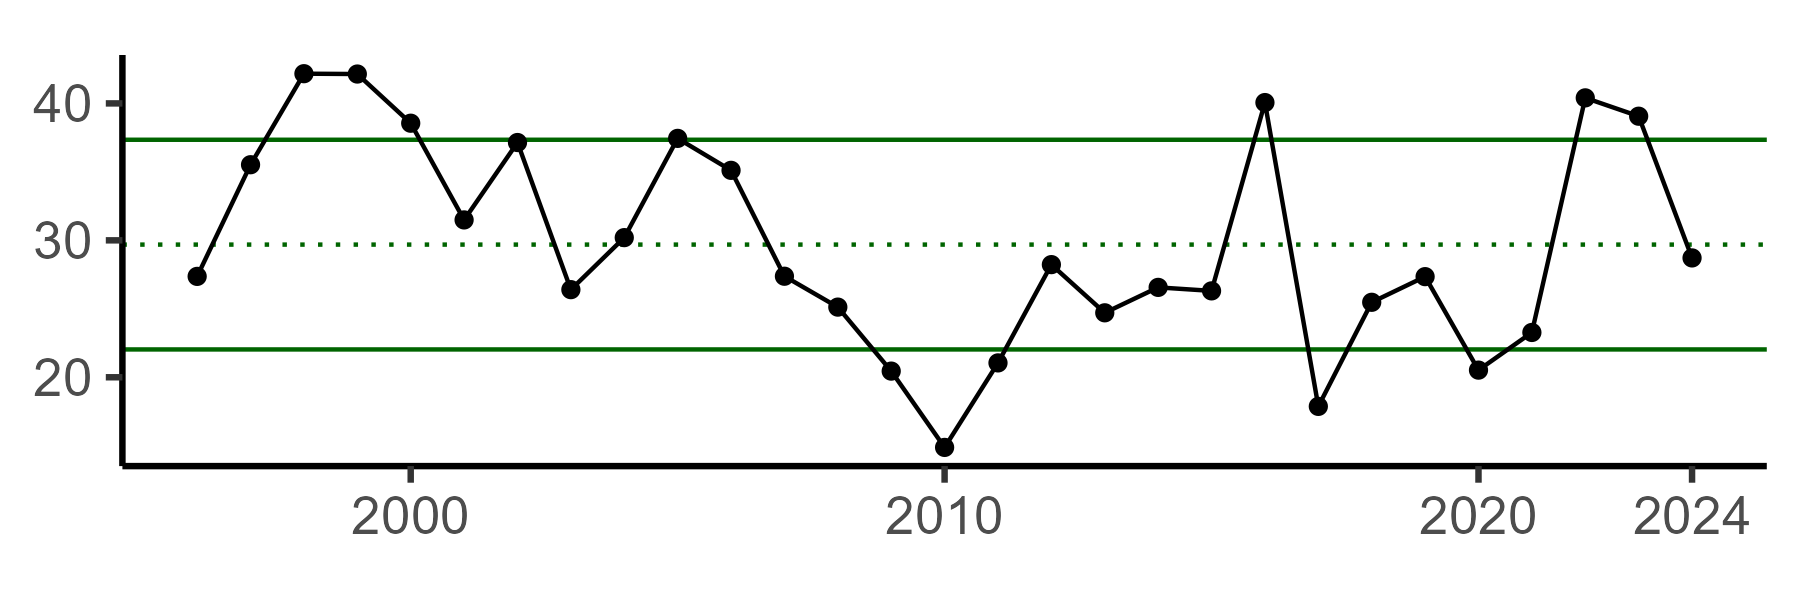
\includegraphics[width=3in, height=1in]{report_card_template_files/figure-pdf/unnamed-chunk-2-1.png}} \\
=======
\multicolumn{1}{!{\color[HTML]{666666}\vrule width 0.75pt}>{\raggedright}m{\dimexpr 0.9in+0\tabcolsep}}{\textcolor[HTML]{000000}{\fontsize{10}{10}\selectfont{\global\setmainfont{Times New Roman}{Commercial\ landings\ (millions\ of\ lbs.)
}}}\textcolor[HTML]{000000}{\fontsize{10}{10}\selectfont{\global\setmainfont{Times New Roman}{\linebreak }}}} & \multicolumn{1}{!{\color[HTML]{666666}\vrule width 0.75pt}>{\raggedright}m{\dimexpr 0.75in+0\tabcolsep}}{\textcolor[HTML]{000000}{\fontsize{10}{10}\selectfont{\global\setmainfont{Times New Roman}{Above\ long\ term\ average}}}} & \multicolumn{1}{!{\color[HTML]{666666}\vrule width 0.75pt}>{\raggedright}m{\dimexpr 3in+0\tabcolsep}}{\textcolor[HTML]{000000}{\fontsize{10}{10}\selectfont{\global\setmainfont{Times New Roman}{Add\ implications\ here\ (3-5\ sentences)}}}} & \multicolumn{1}{!{\color[HTML]{666666}\vrule width 0.75pt}>{\centering}m{\dimexpr 3in+0\tabcolsep}!{\color[HTML]{666666}\vrule width 0.75pt}}{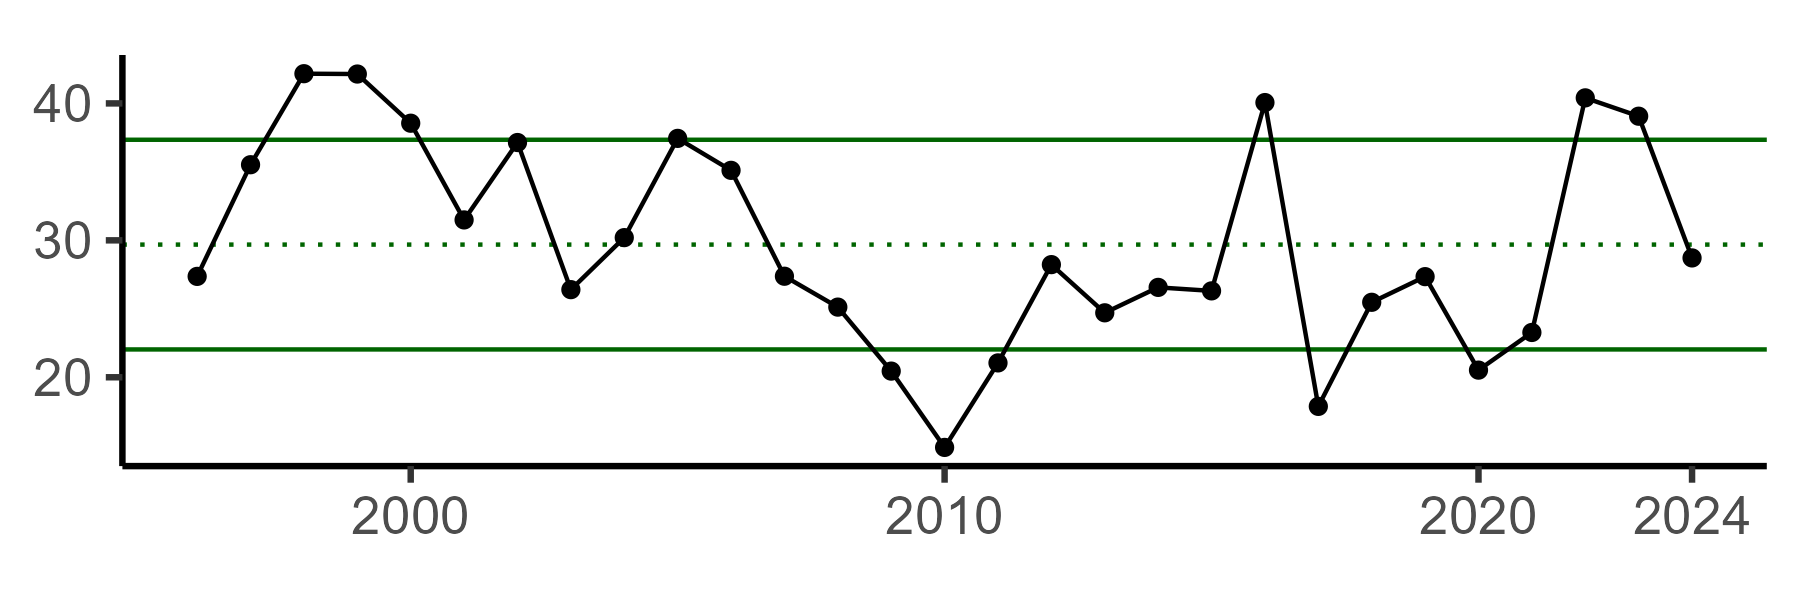
\includegraphics[width=3in, height=1in]{report_card_template_files/figure-pdf/unnamed-chunk-2-1.png}} \\
>>>>>>> 0324c0dd673a4473a6c11ce2d1afb0ef56d69683

\ascline{0.75pt}{666666}{1-4}



<<<<<<< HEAD
\multicolumn{1}{!{\color[HTML]{666666}\vrule width 0.75pt}>{\raggedright}m{\dimexpr 0.9in+0\tabcolsep}}{\textcolor[HTML]{000000}{\fontsize{10}{10}\selectfont{\global\setmainfont{DejaVu Sans}{Number\ of\ commercial\ vessels\ (\#)}}}} & \multicolumn{1}{!{\color[HTML]{666666}\vrule width 0.75pt}>{\raggedright}m{\dimexpr 0.75in+0\tabcolsep}}{\textcolor[HTML]{000000}{\fontsize{10}{10}\selectfont{\global\setmainfont{DejaVu Sans}{Below\ long\ term\ average}}}} & \multicolumn{1}{!{\color[HTML]{666666}\vrule width 0.75pt}>{\raggedright}m{\dimexpr 3in+0\tabcolsep}}{\textcolor[HTML]{000000}{\fontsize{10}{10}\selectfont{\global\setmainfont{DejaVu Sans}{Number\ of\ commercial\ vessels\ has\ been\ steadily\ decreasing\ since\ around\ 2000\ consistent\ with\ decreasing\ fleet\ diversity\ and\ continued\ risk\ to\ fishery\ resilience\ (MAFMC\ FID).}}}} & \multicolumn{1}{!{\color[HTML]{666666}\vrule width 0.75pt}>{\centering}m{\dimexpr 3in+0\tabcolsep}!{\color[HTML]{666666}\vrule width 0.75pt}}{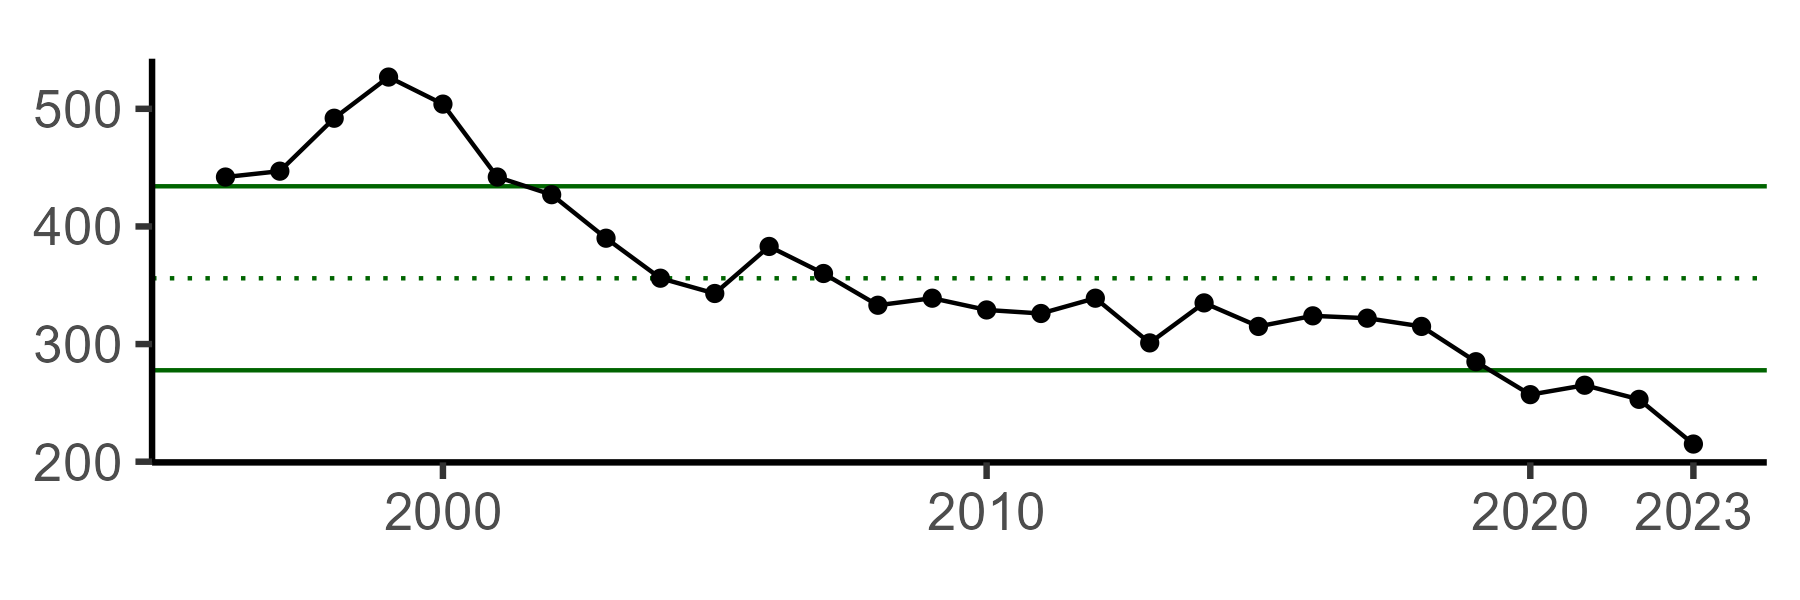
\includegraphics[width=3in, height=1in]{report_card_template_files/figure-pdf/unnamed-chunk-2-2.png}} \\
=======
\multicolumn{1}{!{\color[HTML]{666666}\vrule width 0.75pt}>{\raggedright}m{\dimexpr 0.9in+0\tabcolsep}}{\textcolor[HTML]{000000}{\fontsize{10}{10}\selectfont{\global\setmainfont{Times New Roman}{Number\ of\ commercial\ vessels\ (\#)}}}} & \multicolumn{1}{!{\color[HTML]{666666}\vrule width 0.75pt}>{\raggedright}m{\dimexpr 0.75in+0\tabcolsep}}{\textcolor[HTML]{000000}{\fontsize{10}{10}\selectfont{\global\setmainfont{Times New Roman}{Below\ long\ term\ average}}}} & \multicolumn{1}{!{\color[HTML]{666666}\vrule width 0.75pt}>{\raggedright}m{\dimexpr 3in+0\tabcolsep}}{\textcolor[HTML]{000000}{\fontsize{10}{10}\selectfont{\global\setmainfont{Times New Roman}{Add\ implications\ here\ (3-5\ sentences)}}}} & \multicolumn{1}{!{\color[HTML]{666666}\vrule width 0.75pt}>{\centering}m{\dimexpr 3in+0\tabcolsep}!{\color[HTML]{666666}\vrule width 0.75pt}}{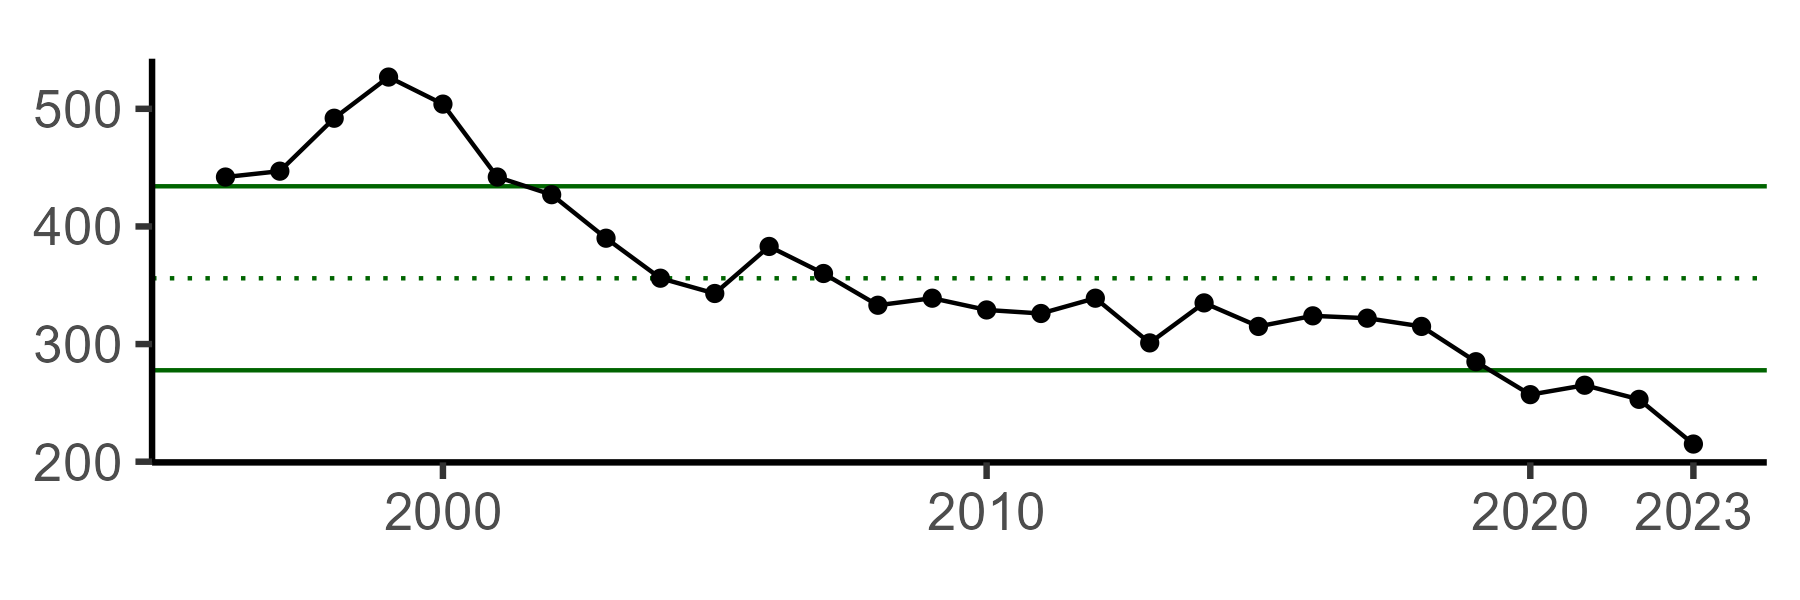
\includegraphics[width=3in, height=1in]{report_card_template_files/figure-pdf/unnamed-chunk-2-2.png}} \\
>>>>>>> 0324c0dd673a4473a6c11ce2d1afb0ef56d69683

\ascline{0.75pt}{666666}{1-4}



<<<<<<< HEAD
\multicolumn{1}{!{\color[HTML]{666666}\vrule width 0.75pt}>{\raggedright}m{\dimexpr 0.9in+0\tabcolsep}}{\textcolor[HTML]{000000}{\fontsize{10}{10}\selectfont{\global\setmainfont{DejaVu Sans}{Commercial\ revenue\ (2024\ USD)}}}} & \multicolumn{1}{!{\color[HTML]{666666}\vrule width 0.75pt}>{\raggedright}m{\dimexpr 0.75in+0\tabcolsep}}{\textcolor[HTML]{000000}{\fontsize{10}{10}\selectfont{\global\setmainfont{DejaVu Sans}{Below\ long\ term\ average}}}} & \multicolumn{1}{!{\color[HTML]{666666}\vrule width 0.75pt}>{\raggedright}m{\dimexpr 3in+0\tabcolsep}}{\textcolor[HTML]{000000}{\fontsize{10}{10}\selectfont{\global\setmainfont{DejaVu Sans}{Average\ Longfin\ ex-vessel\ prices\ in\ 2024\ increased\ slightly\ from\ 2023\ (+10\%),\ but\ commercial\ revenue\ has\ decreased\ from\ 2023\ which\ is\ most\ likely\ driven\ by\ a\ an\ overall\ decrease\ in\ landings\ by\ 23\%\ (MAFMC\ FID).}}}} & \multicolumn{1}{!{\color[HTML]{666666}\vrule width 0.75pt}>{\centering}m{\dimexpr 3in+0\tabcolsep}!{\color[HTML]{666666}\vrule width 0.75pt}}{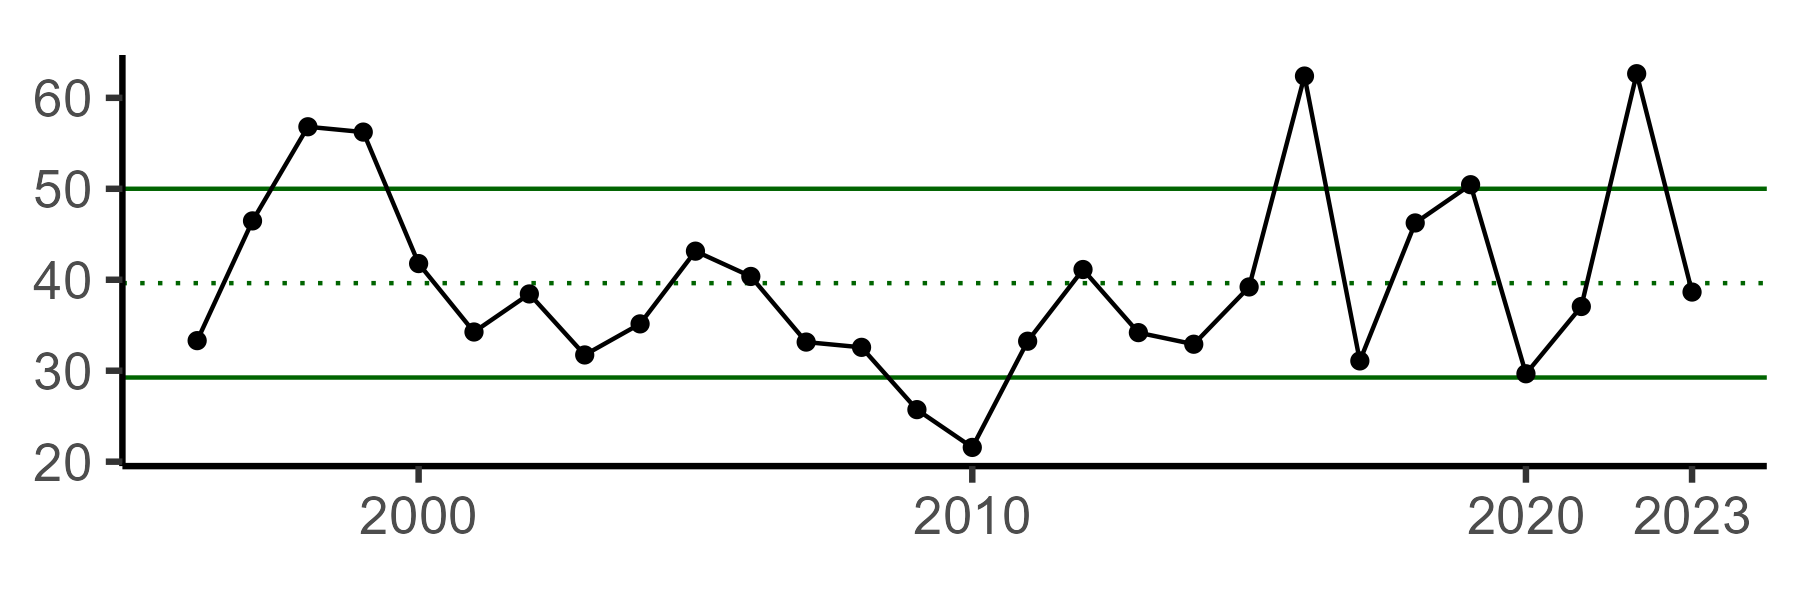
\includegraphics[width=3in, height=1in]{report_card_template_files/figure-pdf/unnamed-chunk-2-3.png}} \\
=======
\multicolumn{1}{!{\color[HTML]{666666}\vrule width 0.75pt}>{\raggedright}m{\dimexpr 0.9in+0\tabcolsep}}{\textcolor[HTML]{000000}{\fontsize{10}{10}\selectfont{\global\setmainfont{Times New Roman}{Commercial\ revenue\ (2023\ USD)}}}} & \multicolumn{1}{!{\color[HTML]{666666}\vrule width 0.75pt}>{\raggedright}m{\dimexpr 0.75in+0\tabcolsep}}{\textcolor[HTML]{000000}{\fontsize{10}{10}\selectfont{\global\setmainfont{Times New Roman}{Near\ long\ term\ average}}}} & \multicolumn{1}{!{\color[HTML]{666666}\vrule width 0.75pt}>{\raggedright}m{\dimexpr 3in+0\tabcolsep}}{\textcolor[HTML]{000000}{\fontsize{10}{10}\selectfont{\global\setmainfont{Times New Roman}{Add\ implications\ here\ (3-5\ sentences)}}}} & \multicolumn{1}{!{\color[HTML]{666666}\vrule width 0.75pt}>{\centering}m{\dimexpr 3in+0\tabcolsep}!{\color[HTML]{666666}\vrule width 0.75pt}}{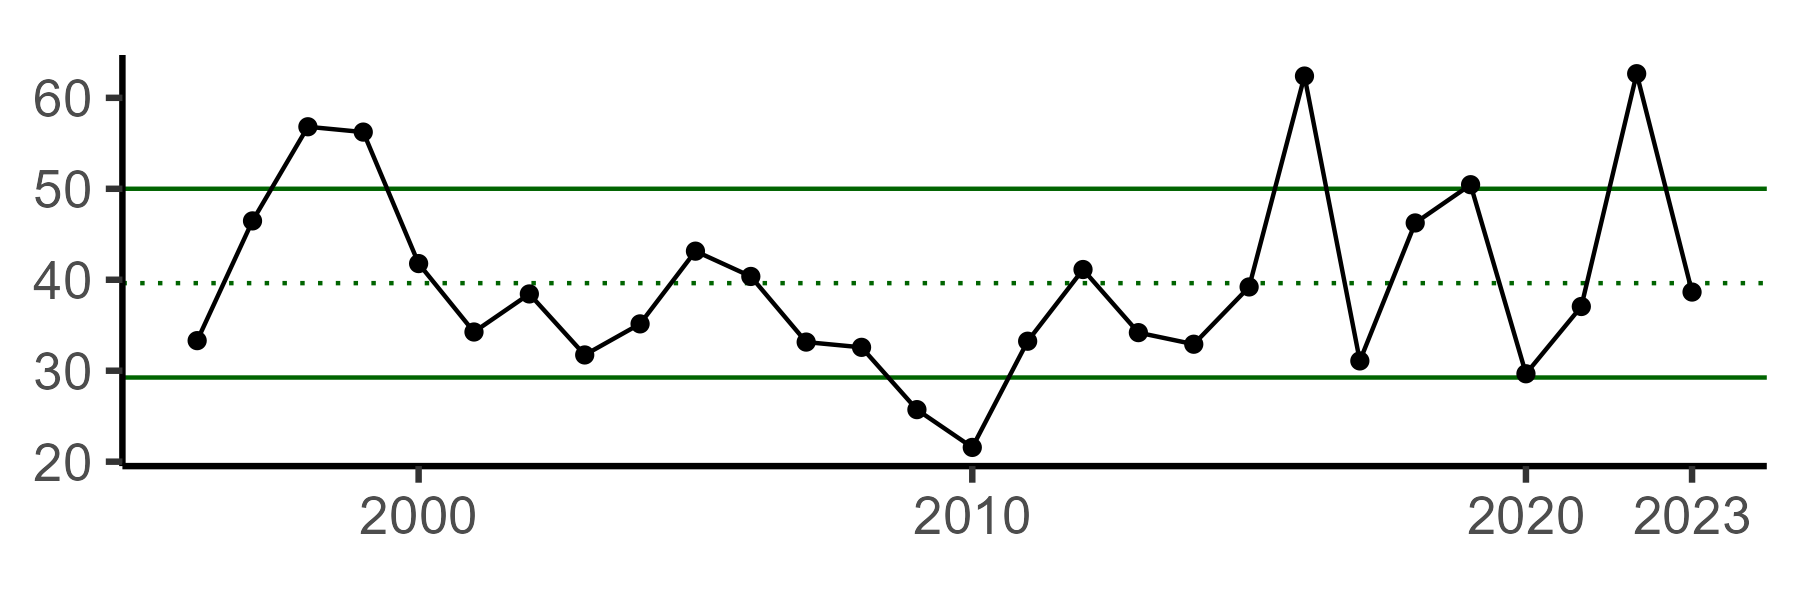
\includegraphics[width=3in, height=1in]{report_card_template_files/figure-pdf/unnamed-chunk-2-3.png}} \\
>>>>>>> 0324c0dd673a4473a6c11ce2d1afb0ef56d69683

\ascline{0.75pt}{666666}{1-4}



<<<<<<< HEAD
\multicolumn{1}{!{\color[HTML]{666666}\vrule width 0.75pt}>{\raggedright}m{\dimexpr 0.9in+0\tabcolsep}}{\textcolor[HTML]{000000}{\fontsize{10}{10}\selectfont{\global\setmainfont{DejaVu Sans}{Western\ Gulf\ Stream\ Index\ (shift\ in\ the\ western\ part\ of\ the\ Gulf\ Stream\ North\ wall:\ mean\ position:\ >0\ =\ more\ northerly,\ <0\ =\ more\ southerly)}}}} & \multicolumn{1}{!{\color[HTML]{666666}\vrule width 0.75pt}>{\raggedright}m{\dimexpr 0.75in+0\tabcolsep}}{\textcolor[HTML]{000000}{\fontsize{10}{10}\selectfont{\global\setmainfont{DejaVu Sans}{Above\ long\ term\ average}}}} & \multicolumn{1}{!{\color[HTML]{666666}\vrule width 0.75pt}>{\raggedright}m{\dimexpr 3in+0\tabcolsep}}{\textcolor[HTML]{000000}{\fontsize{10}{10}\selectfont{\global\setmainfont{DejaVu Sans}{Since\ the\ mid-1990s,\ north\ and\ westward\ shifts\ in\ the\ Gulf\ Stream\ have\ resulted\ in\ an\ increase\ in\ warm\ core\ rings\ and\ deep\ water,\ high\ salinity\ heat\ waves.\ The\ position\ of\ the\ Gulf\ Stream\ influences\ seasonal\ temperature\ and\ water\ mass\ mixing\ dynamics\ that\ affect\ longfin\ squid\ habitat\ suitability,\ temperature-dependent\ growth,\ and\ prey\ availability.}}}} & \multicolumn{1}{!{\color[HTML]{666666}\vrule width 0.75pt}>{\centering}m{\dimexpr 3in+0\tabcolsep}!{\color[HTML]{666666}\vrule width 0.75pt}}{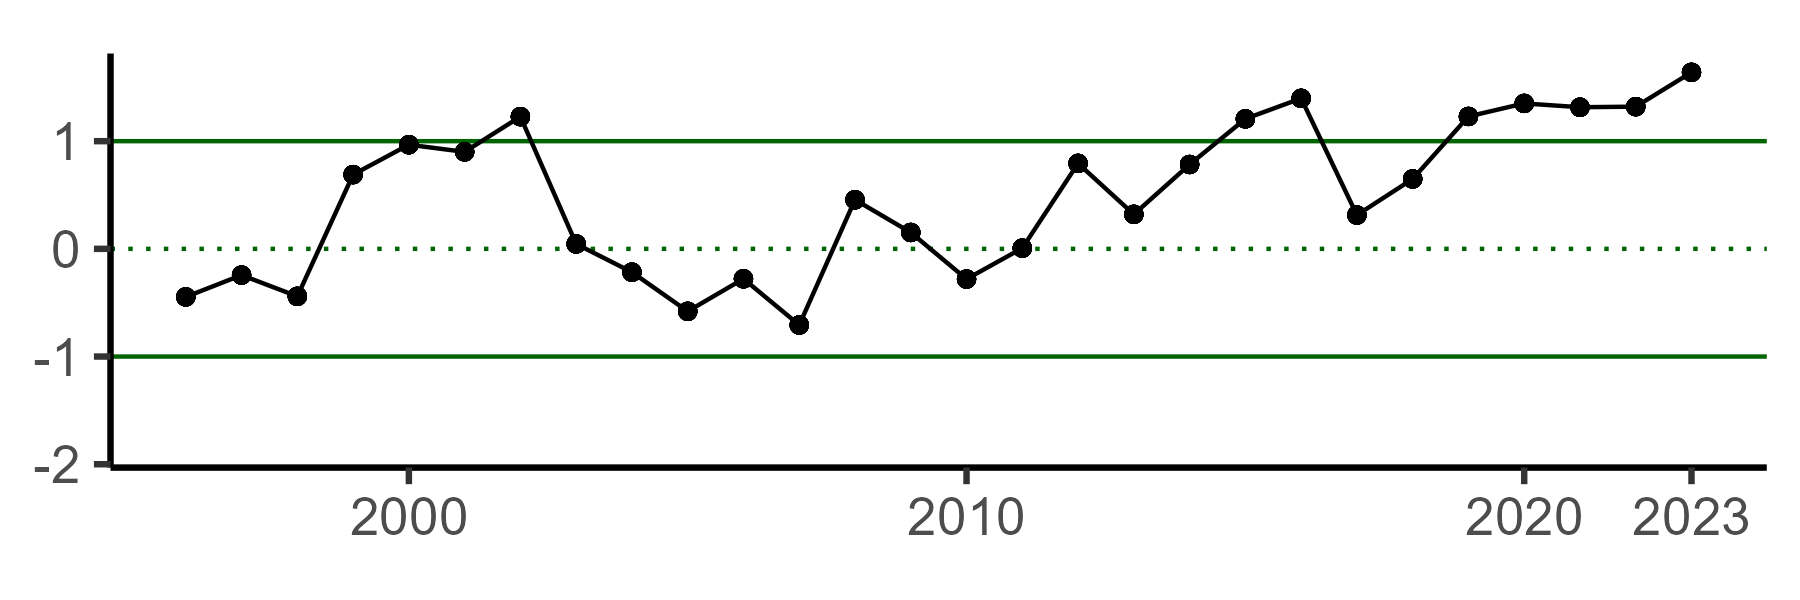
\includegraphics[width=3in, height=1in]{report_card_template_files/figure-pdf/unnamed-chunk-2-4.png}} \\
=======
\multicolumn{1}{!{\color[HTML]{666666}\vrule width 0.75pt}>{\raggedright}m{\dimexpr 0.9in+0\tabcolsep}}{\textcolor[HTML]{000000}{\fontsize{10}{10}\selectfont{\global\setmainfont{Times New Roman}{Western\ Gulf\ Stream\ Index\ (shift\ in\ the\ western\ part\ of\ the\ Gulf\ Stream\ North\ wall:\ mean\ position:\ >0\ =\ more\ northerly,\ <0\ =\ more\ southerly)}}}} & \multicolumn{1}{!{\color[HTML]{666666}\vrule width 0.75pt}>{\raggedright}m{\dimexpr 0.75in+0\tabcolsep}}{\textcolor[HTML]{000000}{\fontsize{10}{10}\selectfont{\global\setmainfont{Times New Roman}{Above\ long\ term\ average}}}} & \multicolumn{1}{!{\color[HTML]{666666}\vrule width 0.75pt}>{\raggedright}m{\dimexpr 3in+0\tabcolsep}}{\textcolor[HTML]{000000}{\fontsize{10}{10}\selectfont{\global\setmainfont{Times New Roman}{Since\ the\ mid-1990s,\ north\ and\ westward\ shifts\ in\ the\ Gulf\ Stream\ have\ resulted\ in\ an\ increase\ in\ warm\ core\ rings\ and\ deep\ water,\ high\ salinity\ heat\ waves.\ The\ position\ of\ the\ Gulf\ Stream\ influences\ seasonal\ temperature\ and\ water\ mass\ mixing\ dynamics\ that\ affect\ longfin\ squid\ habitat\ suitability,\ temperature-dependent\ growth,\ and\ prey\ availability.}}}} & \multicolumn{1}{!{\color[HTML]{666666}\vrule width 0.75pt}>{\centering}m{\dimexpr 3in+0\tabcolsep}!{\color[HTML]{666666}\vrule width 0.75pt}}{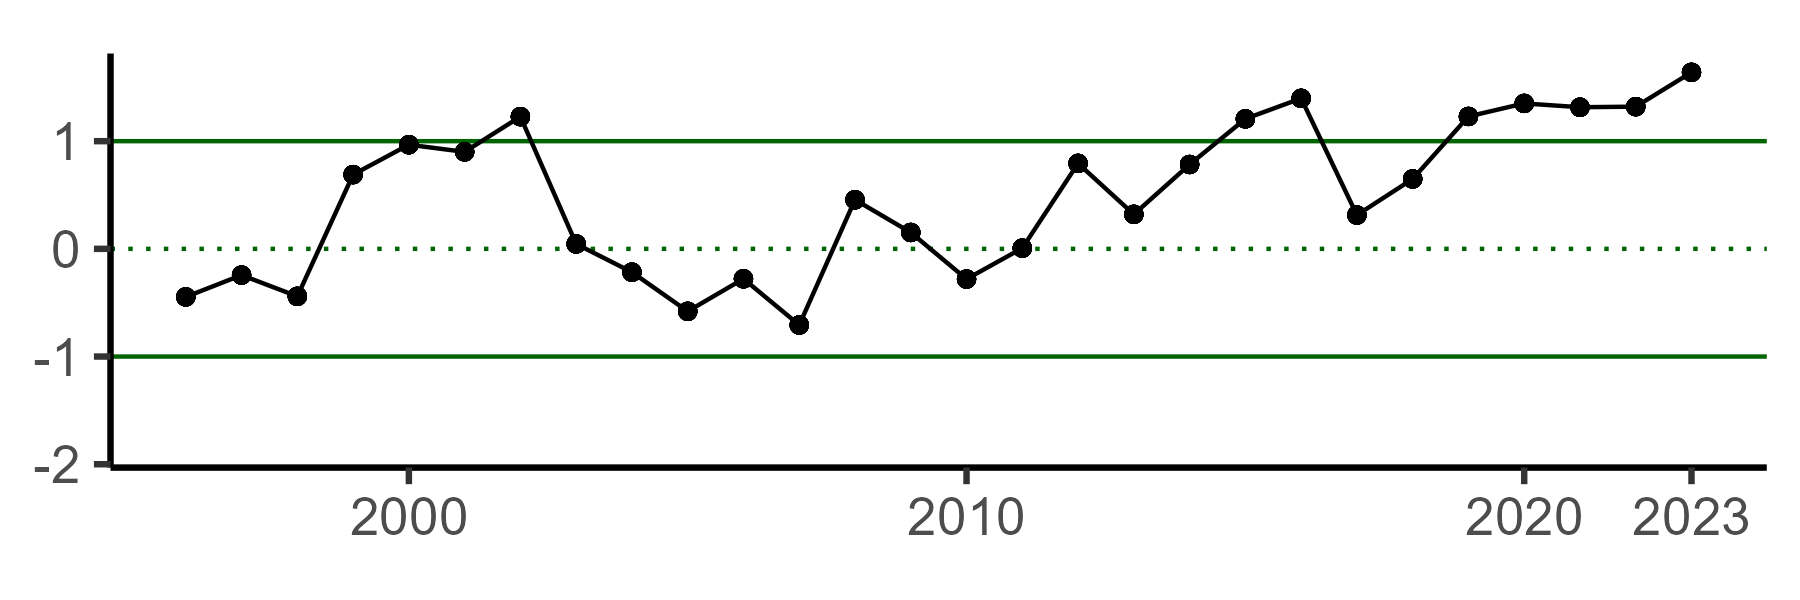
\includegraphics[width=3in, height=1in]{report_card_template_files/figure-pdf/unnamed-chunk-2-4.png}} \\
>>>>>>> 0324c0dd673a4473a6c11ce2d1afb0ef56d69683

\ascline{0.75pt}{666666}{1-4}



<<<<<<< HEAD
\multicolumn{1}{!{\color[HTML]{666666}\vrule width 0.75pt}>{\raggedright}m{\dimexpr 0.9in+0\tabcolsep}}{\textcolor[HTML]{000000}{\fontsize{10}{10}\selectfont{\global\setmainfont{DejaVu Sans}{Bottom\ temperature\ in\ MAB\ and\ SNE(°C)}}}} & \multicolumn{1}{!{\color[HTML]{666666}\vrule width 0.75pt}>{\raggedright}m{\dimexpr 0.75in+0\tabcolsep}}{\textcolor[HTML]{000000}{\fontsize{10}{10}\selectfont{\global\setmainfont{DejaVu Sans}{Above\ long\ term\ average\ (Fall);\ near\ long\ term\ average\ (Spring)}}}} & \multicolumn{1}{!{\color[HTML]{666666}\vrule width 0.75pt}>{\raggedright}m{\dimexpr 3in+0\tabcolsep}}{\textcolor[HTML]{000000}{\fontsize{10}{10}\selectfont{\global\setmainfont{DejaVu Sans}{Longfin\ squid\ seasonal\ distribution\ and\ growth\ rates\ are\ likely\ temperature\ dependent,\ avoiding\ water\ <8°C.\ Inshore\ temperature\ thresholds\ (around\ 14°C)\ initiate\ migration\ of\ squid\ from\ offshore\ overwintering\ habitats.}}}} & \multicolumn{1}{!{\color[HTML]{666666}\vrule width 0.75pt}>{\centering}m{\dimexpr 3in+0\tabcolsep}!{\color[HTML]{666666}\vrule width 0.75pt}}{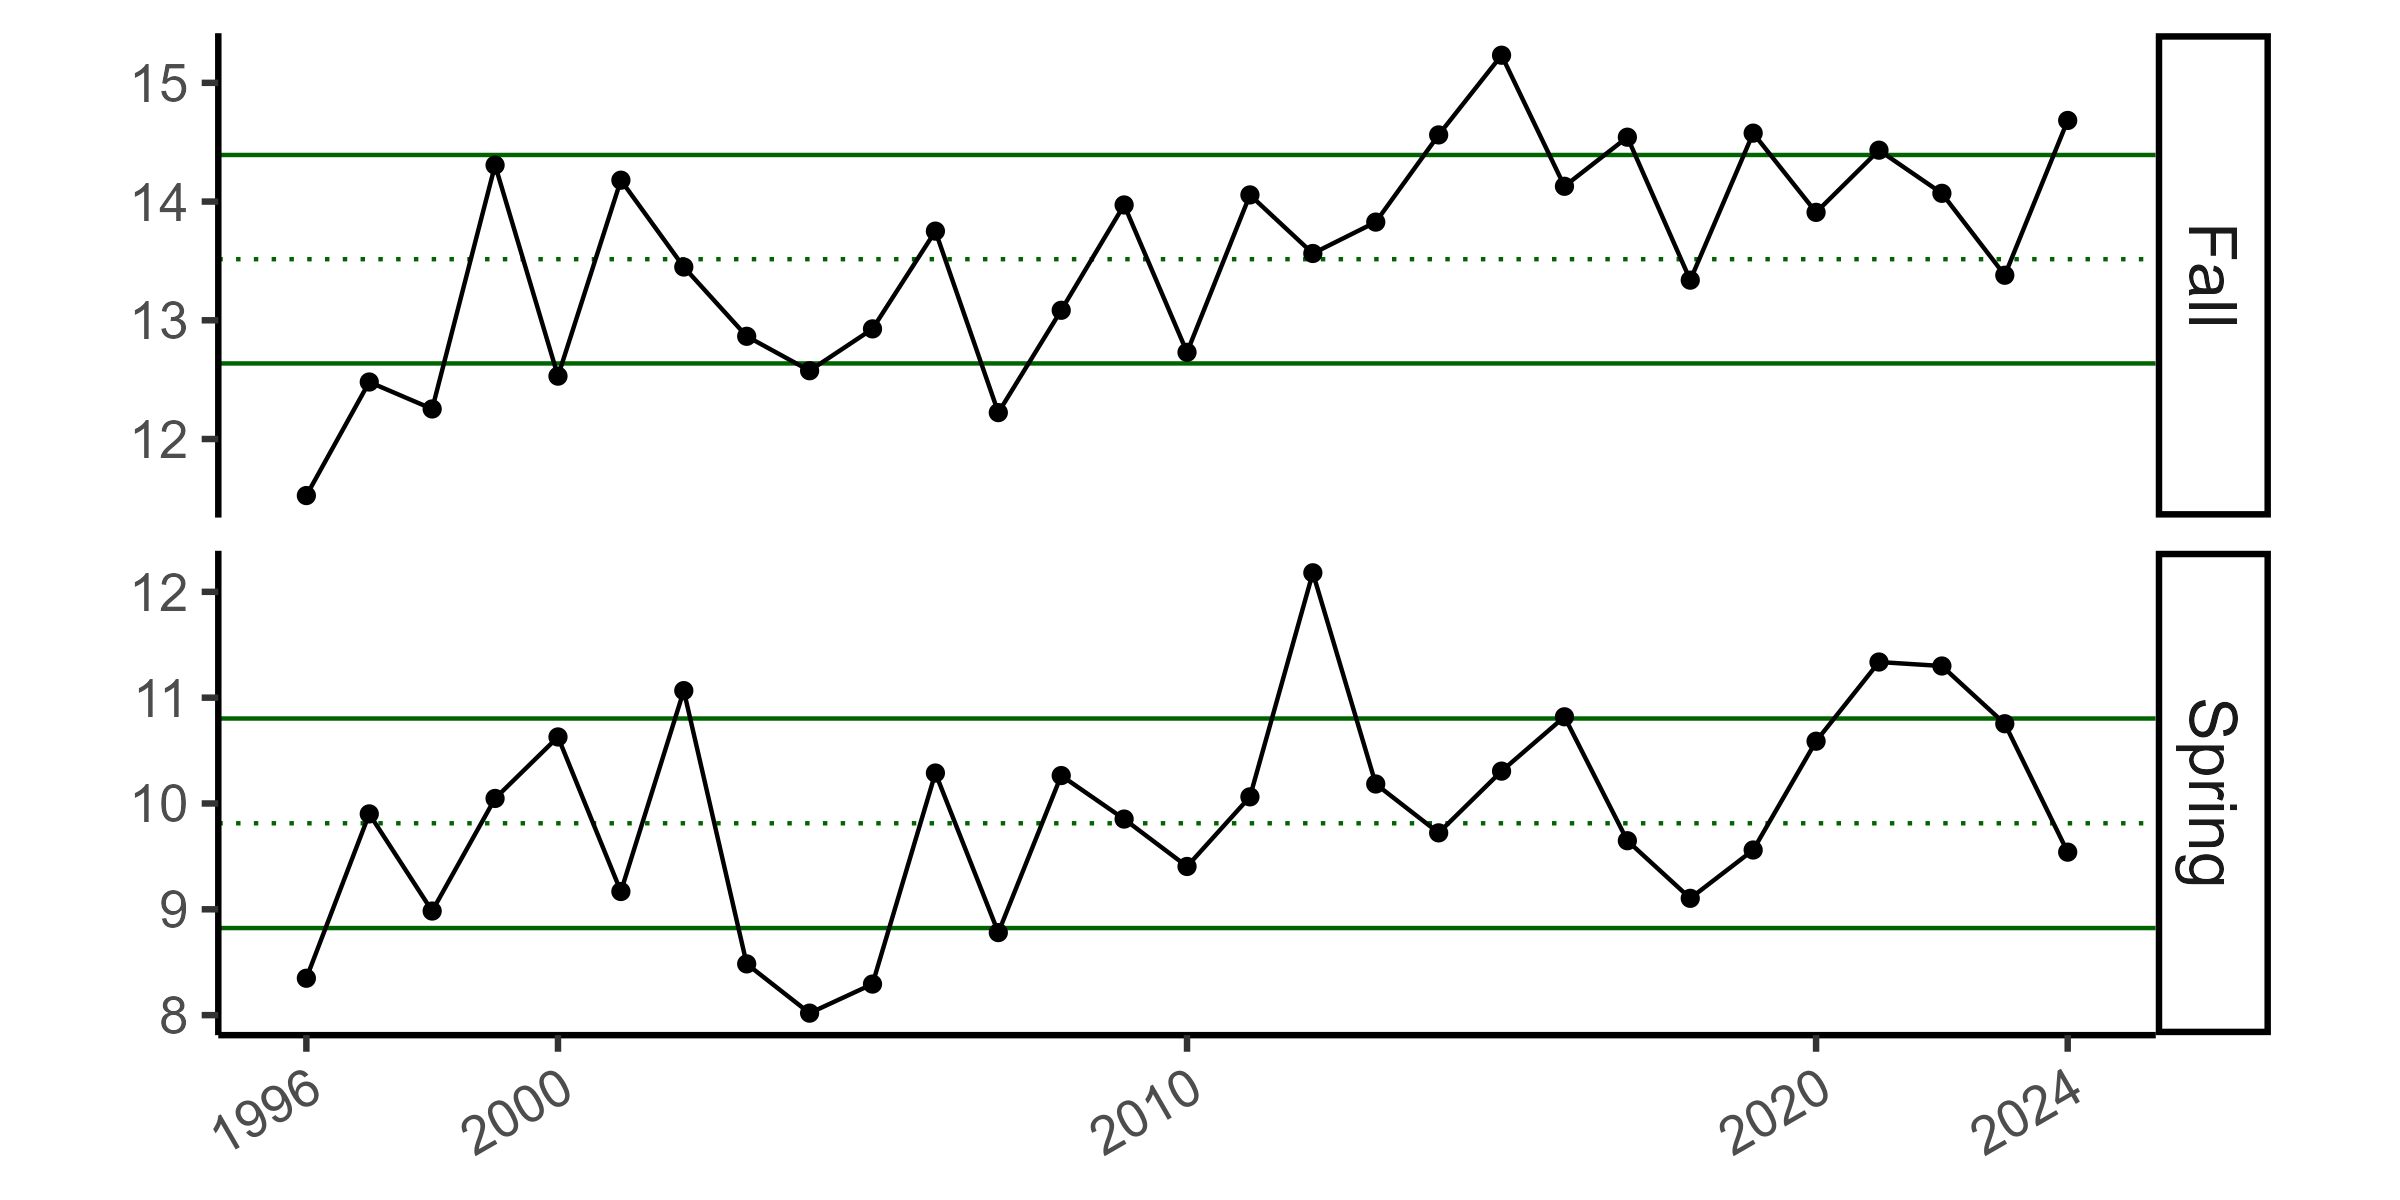
\includegraphics[width=3in, height=1.5in]{report_card_template_files/figure-pdf/unnamed-chunk-2-5.png}} \\
=======
\multicolumn{1}{!{\color[HTML]{666666}\vrule width 0.75pt}>{\raggedright}m{\dimexpr 0.9in+0\tabcolsep}}{\textcolor[HTML]{000000}{\fontsize{10}{10}\selectfont{\global\setmainfont{Times New Roman}{Bottom\ temperature\ in\ MAB\ and\ SNE(°C)}}}} & \multicolumn{1}{!{\color[HTML]{666666}\vrule width 0.75pt}>{\raggedright}m{\dimexpr 0.75in+0\tabcolsep}}{\textcolor[HTML]{000000}{\fontsize{10}{10}\selectfont{\global\setmainfont{Times New Roman}{Above\ long\ term\ average\ (Fall);\ near\ long\ term\ average\ (Spring)}}}} & \multicolumn{1}{!{\color[HTML]{666666}\vrule width 0.75pt}>{\raggedright}m{\dimexpr 3in+0\tabcolsep}}{\textcolor[HTML]{000000}{\fontsize{10}{10}\selectfont{\global\setmainfont{Times New Roman}{Longfin\ squid\ seasonal\ distribution\ and\ growth\ rates\ are\ likely\ temperature\ dependent,\ avoiding\ water\ <8°C.\ Inshore\ temperature\ thresholds\ (around\ 14°C)\ initiate\ migration\ of\ squid\ from\ offshore\ overwintering\ habitats.}}}} & \multicolumn{1}{!{\color[HTML]{666666}\vrule width 0.75pt}>{\centering}m{\dimexpr 3in+0\tabcolsep}!{\color[HTML]{666666}\vrule width 0.75pt}}{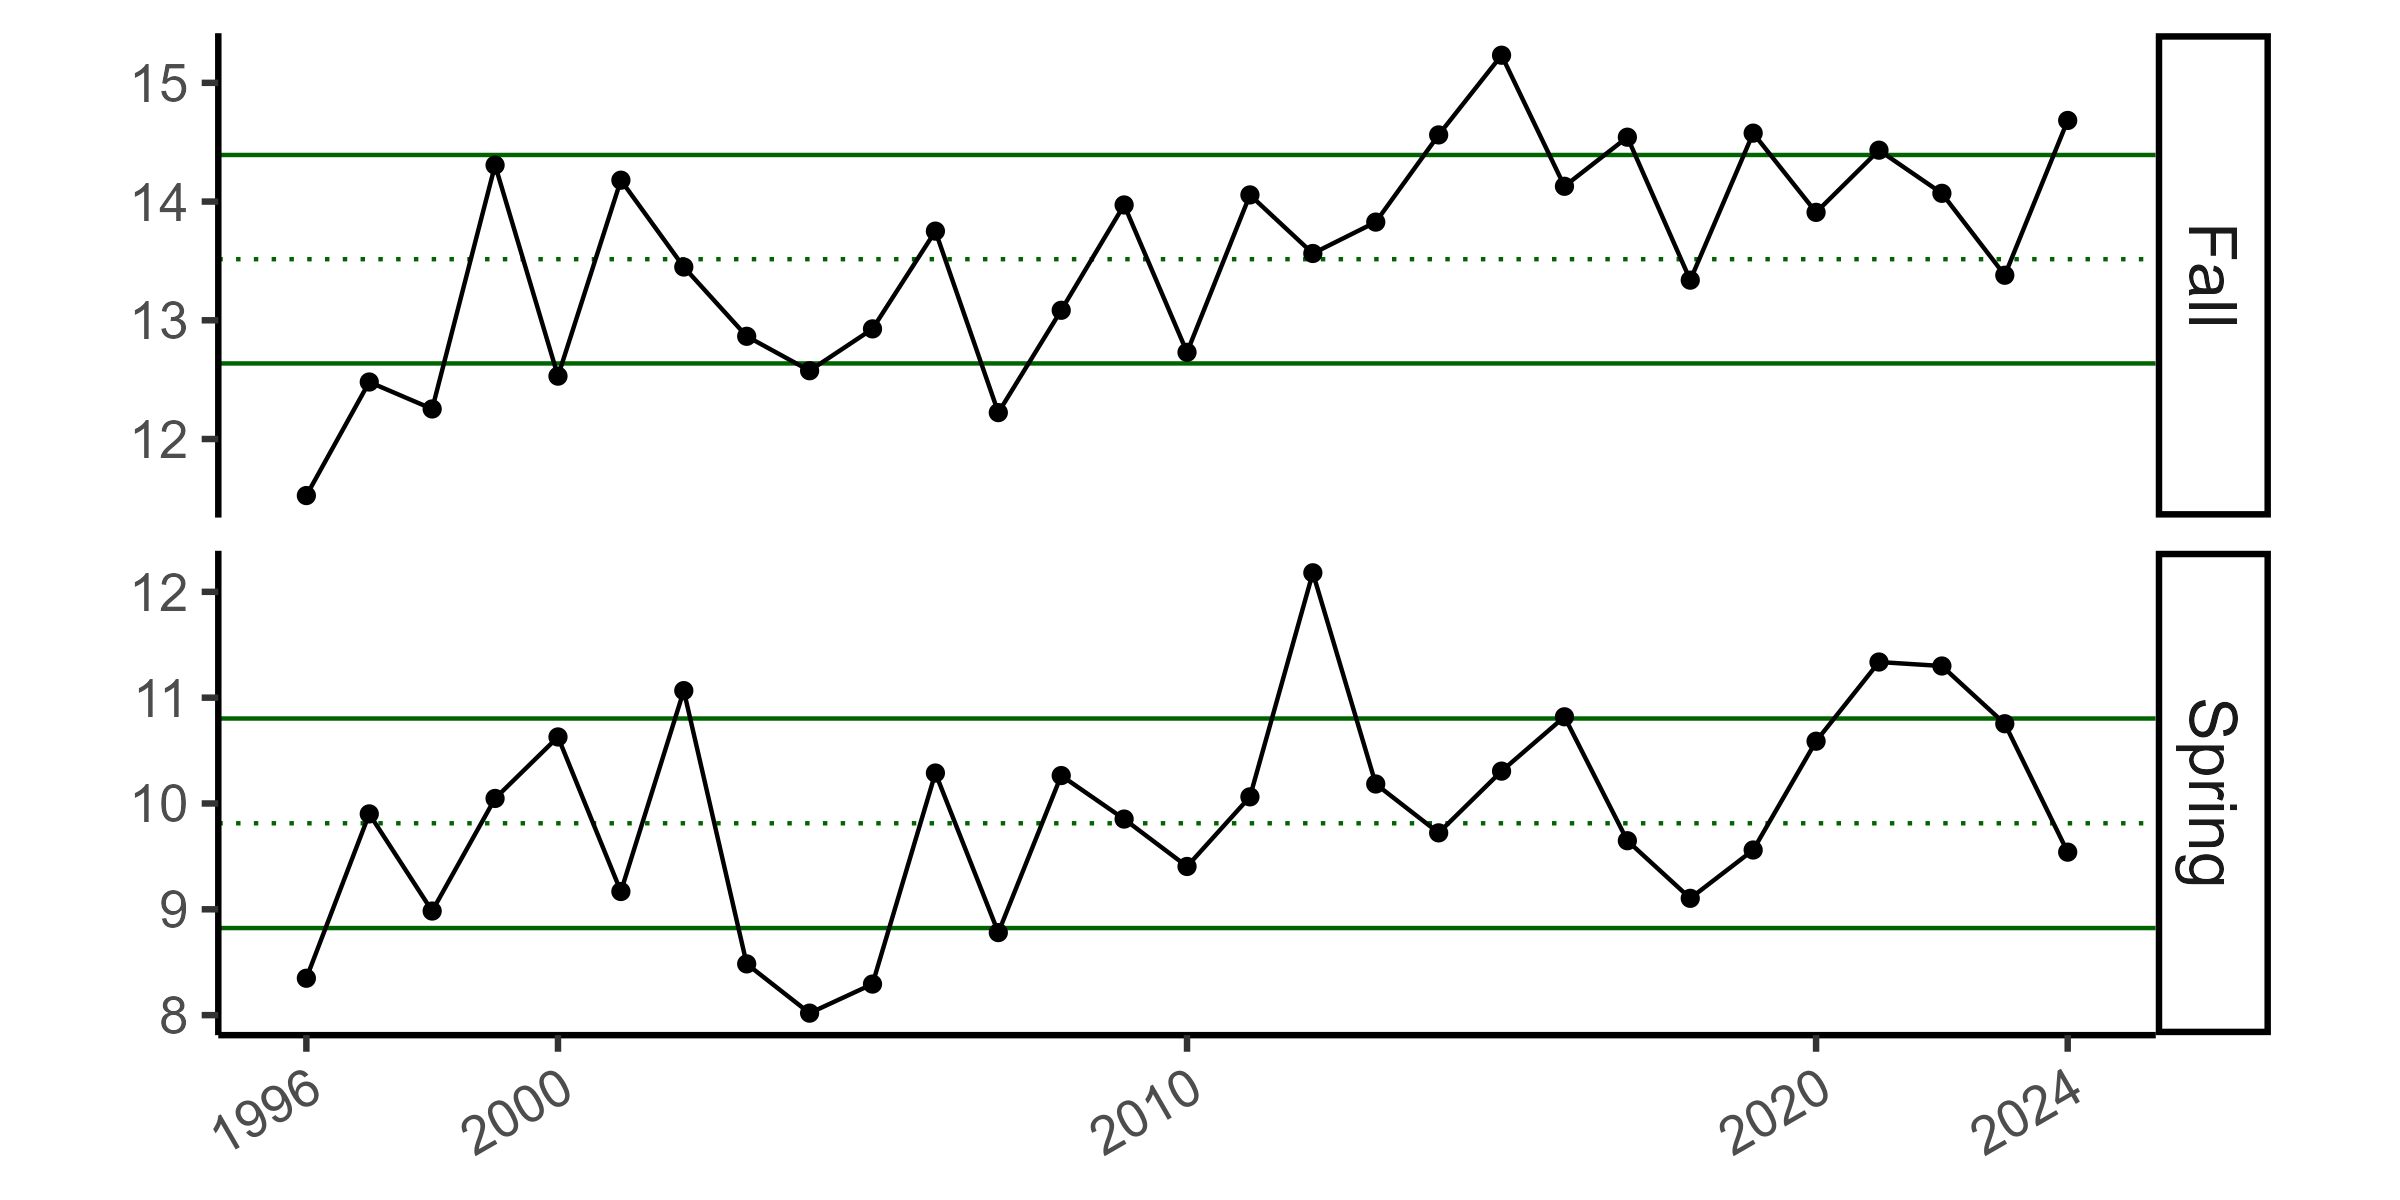
\includegraphics[width=3in, height=1.5in]{report_card_template_files/figure-pdf/unnamed-chunk-2-5.png}} \\
>>>>>>> 0324c0dd673a4473a6c11ce2d1afb0ef56d69683

\ascline{0.75pt}{666666}{1-4}



<<<<<<< HEAD
\end{longtable}
=======
\end{longtable*}
>>>>>>> 0324c0dd673a4473a6c11ce2d1afb0ef56d69683



\arrayrulecolor[HTML]{000000}

\global\setlength{\arrayrulewidth}{\Oldarrayrulewidth}

\global\setlength{\tabcolsep}{\Oldtabcolsep}

\renewcommand*{\arraystretch}{1}

\section{Research Recommendations}

\raggedright

-Expand ecosystem and socioeconomic indicator selection relevant to
longfin squid stock dynamics. Potential ecosystem indicators include
bottom salinity, sea surface temperature, warm core rings, marine
heatwaves, storminess index, indices of food availability, and other
oceanographic indicators relevant to shelf/slope dynamics. Potential
socioeconomic indicators include fuel price, quotas, and ex-vessel
price.

\vspace{0.25cm}

-Analyze indicators against longfin squid metrics, such as a
standardized CPUE index.

\vspace{0.25cm}

-Estimate availability of longfin squid stock to fishery independent
surveys and fishery. Through a seasonal habitat suitability
model/species distribution model.

\vspace{0.25cm}

-Evaluate ecosystem and socioeconomic influences on longfin squid in
<<<<<<< HEAD
reference to the stock assessment and fisheries management
considerations.
=======
reference to the stock assessment and fisheries management consideratio
>>>>>>> 0324c0dd673a4473a6c11ce2d1afb0ef56d69683

\vspace{2.0cm}

\centering

Please contact \url{nefsc.esp.leads@noaa.gov} with any questions or
comments.



\end{document}
